{\bf{Во второй}} главе ставится задача синтеза усовершенствованного алгоритма оценки автокореляционной функции (АКФ) с использованием
быстрого преобразования Фурье. Для верификации синтезированного алгоритма проведено имитационное моделироване.

Точность АР метода напрямую зависит от точности оценки АКФ гармонического сигнала.
Существует несколько способов компенсации шума для АР анализа.
Основным способом повышения точности оценки АКФ является увеличение размера выборки, что в случае фазомодулированного (ФМ) сигнала может быть затруднительным. 

В данной работе предлагается использовать алгоритм увеличения ОСШ методом итеративного вычисления АКФ.
Для снижения вычислительных затрат итеративное вычисление АКФ предлагается реализовывать в базисе Фурье. 

Уточненная оценка АКФ на ${K}$-ом шаге данного алгоритма может быть получена с помощью выражения:
\begin{center}
\begin{equation}
	\label{eq:akf_3}
	\hat{r}_K = F^{-1}\left[ \left| Fx \right| ^{2^K} \right],
\end{equation}
\end{center}
где ${x}$ – вектор входного сигнала после снятия ПСП, ${F}$ – матрица прямого преобразования Фурье,
${F^{-1}}$ - матрица обратного преобразования Фурье.

Схематически алгоритм получения уточненной оценки АКФ на третьем шаге представлен на рисунке \ref{pic:akf_pic}.
\begin{figure}[h]
	\center\scalebox{0.8}{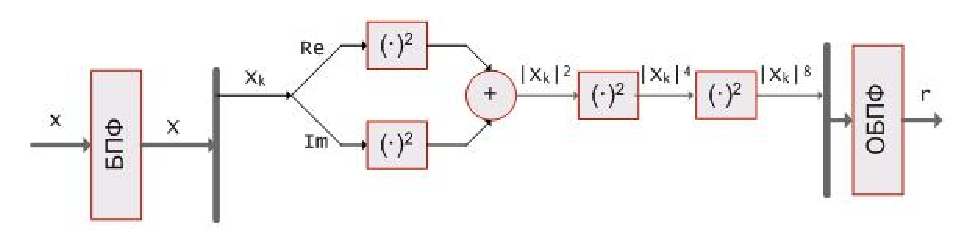
\includegraphics[width=1\linewidth]{akf_fft.eps}}
	\caption{Усовершенствованный итеративный алгоритм получения АКФ}
	\label{pic:akf_pic}
\end{figure}

Количество умножений необходимых для оценки АКФ при помощи прямого метода:
\begin{center}
\begin{equation}
	%\label{eq:}
	OP_{ACF} = 3N^2.
\end{equation}
\end{center}

Количество умножений необходимых для оценки усовершенствованным итеративным алгоритмом получения АКФ: \begin{center}
\begin{equation}
	%\label{eq:}
	OP_{ACF\_FFT} = 8NlogN + (k+2)N.
\end{equation}
\end{center}

%ОСШ в оценке АКФ по мощности можно вычислить по известной формуле:
%\begin{center}
%\begin{equation}
%	\label{eq:akf_max_eq}
%	R_s=2 B T R_e \frac{1}{2+1/R_e}
%\end{equation}
%\end{center}
%где ${R_s}$ - оценка ОСШ для АКФ, ${R_e}$ - ОСШ исходного сигнала, ${T}$ - длинна выборки (сек), ${B}$ -  ширина спектра сигнала.

%На рисунке \ref{pic:gps_spectrum} представлен спектр после повторной модуляции ПСП. 
% FIXME сделать сайд бай сайд до и после пересчета АКФ
В случае наличия интерференции, представляющей собой окрашенный шум, оценка параметрическим методом даст смещенное значение.
Применение усовершенствованного алгоритма итеративного вычисления АКФ позволяет получить ярко выраженный пик в спектральной области,
а СПМ приобретает симметричный вид, что позволяет использовать АР модель второго порядка для получения несмещенной оценки частоты
широкополосного сигнала.

После трех 
итераций предлагаемого алгоритма пик, соответствующий гармонической компоненте, существенно вырастает - рисунок \ref{pic:GPS_spectrum_iter3}.
\begin{figure}[h]
	\center\scalebox{0.8}{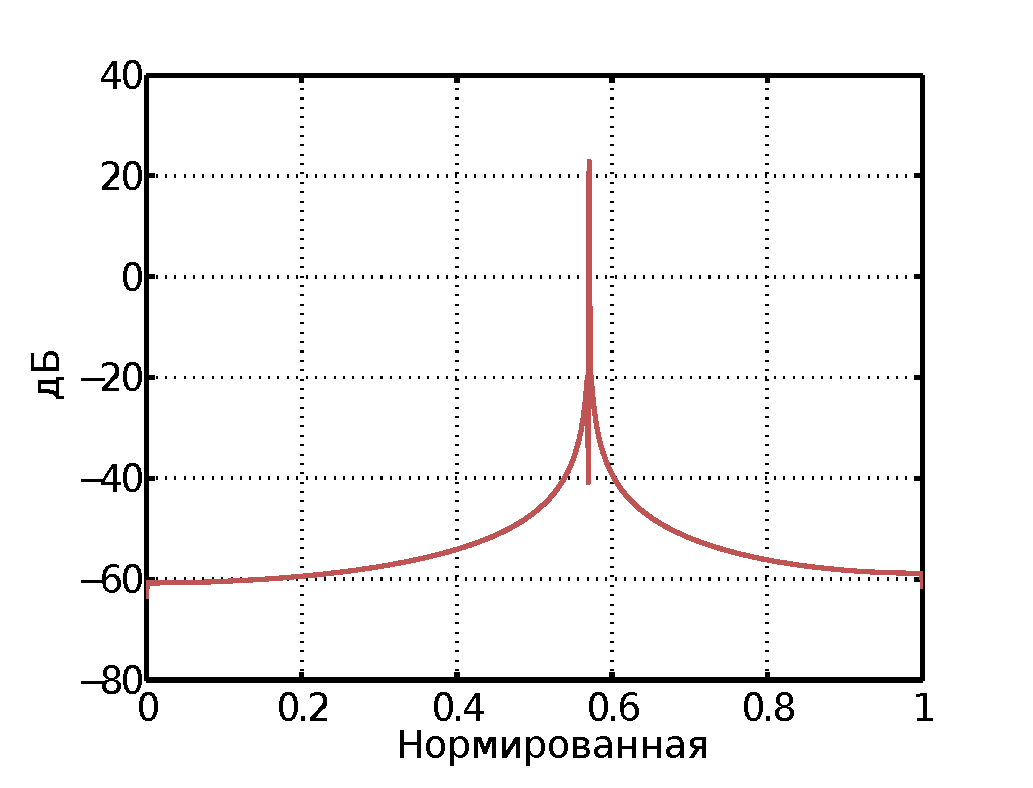
\includegraphics[width=1\linewidth]{GPS_spectra_iter3.eps}}
	\caption{СПМ сигнала после 3 итерации уточнения АКФ}
	\label{pic:GPS_spectrum_iter3}
\end{figure}

